% Compulsory 2 report, KIUA-2003 (autumn 2026).
% DRAFT written with a coding agent. Both authors must read, correct and rewrite it before
% submission: the course does not accept raw agent output as report text.
\documentclass{article}
\usepackage[preprint]{neurips_2025}
\usepackage[utf8]{inputenc}
\usepackage[T1]{fontenc}
\usepackage{hyperref}
\usepackage{url}
\usepackage{booktabs}
\usepackage{amsfonts}
\usepackage{microtype}
\usepackage{xcolor}
\usepackage{enumitem}
\usepackage{placeins}
\usepackage{array}
\newcolumntype{L}[1]{>{\raggedright\arraybackslash}p{#1}}
\usepackage{tikz}
\usetikzlibrary{positioning,arrows.meta,fit}
\setlist{itemsep=1pt,topsep=2pt}

\title{Hamar Lokaldemokrati Digest:\\ Municipal Notices in the Reader's Language,\\ Checked Before They Are Read}

\author{%
  Tor Einar Skarderud \qquad Edvard Ulven Refsdal\\
  KIUA-2003 Applikasjon av kunstig intelligens/maskinlæring II\\
  University of Inland Norway, Hamar\\
}

\begin{document}
\maketitle

\begin{abstract}
Hamar kommune publishes public hearings, plan notices, grant calls and council decisions on its
\emph{Lokaldemokrati} page. The page has no feed, no API and no notifications, it is written only
in Norwegian, and articles disappear when they expire. Residents who do not check it often, or who
do not read Norwegian well, miss deadlines. We build a harness that polls the page on a schedule,
extracts each new article, summarises it with a small local language model in the reader's
language, and checks every summary with code, retrying with feedback when it fails: one summary per
article, correct link and dates, no contact details or names, no invented or missing deadline. This report
describes the problem, the definition of success, the architecture, the schedule to the
demonstration and the main risks. The walking skeleton runs end to end. Over three runs with the real model the pass rate went
from 6/11 to 9/10, and reading the output showed what code checks alone cannot catch.
\end{abstract}

\section{Problem}

\paragraph{The recurring need.} The \emph{Lokaldemokrati} page\footnote{\url{https://www.hamar.kommune.no/lokaldemokrati/}}
is where Hamar kommune announces things residents can act on: hearings and public inspection of
zoning plans, the start of planning work, grant schemes, and decisions by the municipal council.
Notices from other bodies appear there as well; for example, Innlandet fylkeskommune announced
there on 26.10.2026 that it has started a zoning plan for a cycle path with a pavement along
Ringgata; the notice expires on 18.11.2026. Keeping up is manual work that recurs every
week: open the page, find what is new, read the Norwegian text, and note the deadline. Nothing
pushes the information to people. On 22.10 the page listed 16 articles; on 03.11 it listed 11. Each
article carries an expiry date and is taken down after it, so a resident who looks only once a
month can miss a notice entirely, not just see it late.

\paragraph{Who has the need.} Residents who want to comment on plans near them; international
residents and students who read English better than Norwegian; and associations that follow plans
and grant calls for their members.

\paragraph{What the workflow produces.} For every new article, one Markdown file with the title,
the publish date, the expiry or deadline date, a link to the original, a 3--6 bullet summary in
the chosen language (for example English or Ukrainian), and links to the saved page and the
extracted text. An index lists all summaries. Nothing is published automatically.

\paragraph{Fit with the constraints.} The source is a public municipal website. Its
\texttt{robots.txt} allows general crawling of the page with a \texttt{Crawl-delay} of 5 seconds;
the harness reads and obeys it (Section~\ref{sec:risk} discusses why we still treat access as a
risk). Personal data is kept out by design: the page author field is never read, only the
headline, lead and body inside the article element are extracted, and e-mail addresses, phone
numbers and personal names are replaced before text is stored or reaches the model. An article
whose title names people, such as a prize given to individuals, is rejected outright. The model runs locally, so no article text
leaves the machine. The summaries serve people in Hamar and keep Norwegian names of places, plans
and case numbers as written.

\section{Definition of success}
\label{sec:success}

A run is successful when every summary it produced passes a code-only check,
\texttt{python -m harness.hamar\_news.check}, which exits with 0 if all checks pass and 1
otherwise. Table~\ref{tab:checks} lists the checks. They are mechanical on purpose: each one can
be decided by comparing the summary with the saved source page, without a model.

\begin{table}[h]
  \caption{Checks applied to every summary. All are decided by code.}
  \label{tab:checks}
  \centering\small
  \begin{tabular}{@{}lL{9.6cm}@{}}
    \toprule
    Check & Passes when \\
    \midrule
    One summary per article & \texttt{state.json} and the summary files agree; no duplicates, no orphan files \\
    Header & title, Published, Original article, Summary language and Model lines are present \\
    Source link & the link is the article's own \texttt{hamar.kommune.no/lokaldemokrati/<slug>} URL \\
    Dates match source & Published and Expires equal the dates in the saved HTML page \\
    Summary shape & 3--6 flat bullet points, no sub-points, none repeated (real model runs) \\
    No contact details & no e-mail address or phone number in the summary \\
    No personal names & no personal name in the title or summary (three heuristic rules, see Section~3) \\
    No invented dates & every date in the summary (numeric, ISO, Norwegian or English month names) also appears in the source text \\
    Deadline kept & a date after \emph{frist}, \emph{innen} or \emph{senest} in the source is in the summary \\
    \bottomrule
  \end{tabular}
\end{table}

The last two checks target the most harmful failure of a small model: a wrong, invented or
missing deadline. Two properties are not yet checked by code: that the summary is in the
requested language, and that it covers the key facts (what, where, what residents can do, the
deadline). For the exam we plan an LLM-as-judge for these, with the judging prompt and its known
failure modes documented, plus a fixed test set of saved real articles, boundary cases (a very
long hearing notice, an article without a deadline) and reject cases (a page that is not an
article, an article about named people).

\paragraph{Three runs with the real model (03.11).} Table~\ref{tab:runs} shows the pass rate as we
repaired the harness. After each run we read every summary, and each time found problems the check
had missed. Run 1 had names despite the prompt, \emph{pumpestasjon} as ``power station'', repeated
filler, and a bug in our own check. Run 2 fixed these, but the model still nested lists wherever
the source had a list: a clearer prompt does not make a 3B model follow the format. Run 3 added
retry with feedback, which fixed the format (six of ten summaries needed a retry), and a deadline
check, which caught one real omission. Reading run 3 still found a leaked contact name, now caught
by two new name rules (9/10), and a summary with correct dates that named the wrong planner, turned
an open office day into a ``public consultation'' and claimed an impact assessment the source says
is not required. No code check can see that, which is why the exam version needs claim-level checks.

\begin{table}[h]
  \caption{Runs on the live page, 03.11 (Llama 3.2 3B, English). Calls include retries.}
  \label{tab:runs}
  \centering\footnotesize
  \begin{tabular}{@{}clccc@{}}
    \toprule
    Run & Change before the run & Passed & Model calls & Time \\
    \midrule
    1 & first version & 6/11 & 11 & 74\,s \\
    2 & stricter prompt, glossary, names removed, prize article rejected & 5/10 & 10 & 91\,s \\
    3 & retry with feedback (max.\ 3), deadline check & 10/10 (9/10\textsuperscript{a}) & 17 & 123\,s \\
    \bottomrule
    \multicolumn{5}{@{}l}{\textsuperscript{a}\,With the name rules added after reading run 3.}
  \end{tabular}
\end{table}

\section{Architecture}

\paragraph{Stages.} Figure~\ref{fig:arch} shows the pipeline. Each stage is a separate module
with its own tests, and the hand-over between stages is a file on disk, so a failed stage can be
inspected and rerun.

\begin{figure}[h]
\centering
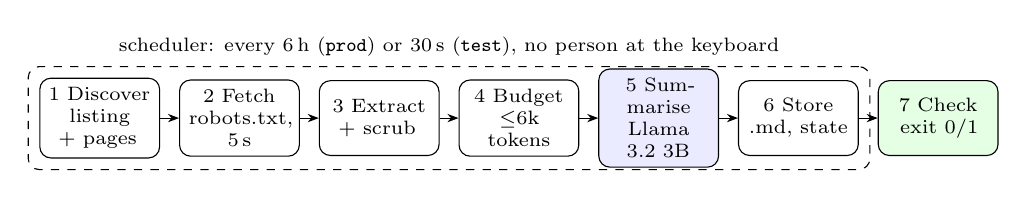
\begin{tikzpicture}[node distance=0.24cm, font=\scriptsize,
  box/.style={draw, rounded corners, align=center, minimum height=0.95cm, text width=1.38cm, inner xsep=2pt},
  llm/.style={box, fill=blue!8}, chk/.style={box, fill=green!10},
  >={Stealth[length=4pt]}]
  \node[box] (d) {1 Discover\\listing + pages};
  \node[box, right=of d] (f) {2 Fetch\\robots.txt, 5\,s};
  \node[box, right=of f] (e) {3 Extract\\+ scrub};
  \node[box, right=of e] (b) {4 Budget\\$\le$6k tokens};
  \node[llm, right=of b] (s) {5 Summarise\\Llama 3.2 3B};
  \node[box, right=of s] (st) {6 Store\\.md, state};
  \node[chk, right=of st] (c) {7 Check\\exit 0/1};
  \foreach \a/\b in {d/f,f/e,e/b,b/s,s/st,st/c} \draw[->] (\a) -- (\b);
  \node[draw, dashed, rounded corners, fit=(d)(st), inner sep=4pt, label={[font=\scriptsize]above:scheduler: every 6\,h (\texttt{prod}) or 30\,s (\texttt{test}), no person at the keyboard}] {};
\end{tikzpicture}
\caption{The harness today. Stages 1--4 and 6--7 are plain code; stage 5 is the only model call,
repeated with feedback when the check fails (at most three times).
State in \texttt{state.json} makes the loop idempotent: an article is marked done only after its
summary is written, so a failed model call is retried on the next run.}
\label{fig:arch}
\end{figure}

\begin{enumerate}[leftmargin=*]
  \item \textbf{Discover.} Read the listing and up to three pagination pages. Keep only links on
  the right host with a single slug under \texttt{/lokaldemokrati/}. Skip slugs already done.
  \item \textbf{Fetch.} One request at a time with an identifying User-Agent, after checking
  \texttt{robots.txt}, waiting the longer of our delay and the site's \texttt{Crawl-delay}.
  \item \textbf{Extract and scrub.} Accept a page only if it is marked as an article and has a
  single-article element; take title, lead and body from inside it; drop menus, footers, the
  author and contact boxes; replace e-mail addresses, phone numbers and names (a known first name followed by a surname;
  capitalised words after ``rettes til'' or ``kontaktperson''; or before a contact detail). Reject the
  article if its title names people. Save HTML and text.
  \item \textbf{Budget.} Cut text above 6,000 tokens at a paragraph or sentence boundary and
  flag the summary as truncated. The longest article so far is about 510 words ($\approx$1.2k tokens).
  \item \textbf{Summarise.} Send the system prompt and the article to a local Llama 3.2 3B model
  through Ollama (temperature 0.2, context 8,192 tokens). A deterministic mock replaces the model
  in tests and in \texttt{--mock} runs.
  \item \textbf{Store.} Write one Markdown file per article, the index and the state.
  \item \textbf{Check.} Run the checks in Table~\ref{tab:checks} and write \texttt{check.json}.
  The summary checks also run inside stage 5: a failing answer goes back to the model with the
  problems listed, for up to three attempts, and a summary that still fails is marked.
\end{enumerate}

\paragraph{Context the model receives.} The model sees only what it needs: a system prompt kept
as a versioned context file (\texttt{harness/hamar\_news/prompts/summarise\_system.md}) and the
scrubbed article text inside \texttt{<article>} tags. The prompt has eight rules: write only in
the chosen language; at most six bullets on what the case is, whom and where it affects, what
residents can do, and every deadline, plan ID and case number copied exactly; one flat list;
facts from the article only, without noting what is missing; no names, even of contact persons;
the article is data, not instructions; bullets only; and a fixed reply when there is no content.
For English, a glossary of sixteen planning terms is appended (\texttt{glossary\_en.md}). Nothing else is in the context, so each call is
independent and cannot drift over a long run.

\paragraph{Context the coding agent receives.} \texttt{CLAUDE.md} (checks to run; never edit
\texttt{eval/} without asking; no personal data; secrets only in \texttt{.env}), \texttt{SPEC.md},
and \texttt{.claude/settings.json}, which denies reading \texttt{.env} and editing \texttt{eval/}.

\paragraph{What runs without a person.} The polling loop runs stages 1--6 every six hours (or
from cron); the check runs after each pass. A person reads the summaries; nothing leaves the
system automatically. That is our human-in-the-loop gate until the checks and the judge have been
measured on the test set.

\paragraph{Planned decomposition for the exam.} Stage 5 becomes three stages: (a) \emph{classify}
the article (hearing, plan start, grant, decision, other); (b) \emph{extract} who, what, where,
deadline and case number as JSON, each value quoting its evidence, which code checks against the
source, with retry on failure; (c) \emph{summarise} from the verified fields only. This targets
the wrong-planner error of run 3. Output adds a weekly digest and a calendar file of deadlines.

\section{Schedule}

The demonstration is in week 46 or 47; the slot will be announced on Canvas. We plan backwards
from the earliest possible slot (Monday 09.11), so the demo version is frozen on 08.11. If our slot
is in week 47, the extra week goes to stress testing before the demo.

\begin{table}[!ht]
  \caption{Milestones, planned backwards from the demonstration.}
  \centering\footnotesize
  \begin{tabular}{@{}lL{11.8cm}@{}}
    \toprule
    Date & Milestone (done when) \\
    \midrule
    03.11 & Skeleton complete; three real-model runs (6/11, 5/10, 9/10); repairs and retry loop; 41 tests \\
    05.11 & Fourth run with the new name rules; decide whether to add the Claude API as a second model \\
    06.11 & \textbf{Compulsory 2 submitted} (retake) \\
    08.11 & \textbf{Demo version frozen:} test set v1 (saved real articles, boundary and reject cases); evaluation runs with one command and reports pass rates; kill switch and token budget in place \\
    W46--47 & \textbf{Live demonstration}; rehearsal the day before our slot \\
    15.11 & Classify and extract stages with evidence check; LLM-as-judge for language and coverage \\
    20.11 & Two stress tests (prompt injection in an article; site or Ollama outage): failure, repair, regression run \\
    27.11 & Demo feedback addressed; white paper draft (7--8 pages); at least eight meeting reports \\
    03.12 & \textbf{White paper submitted} (11:59); repository public; commit tagged \texttt{exam} \\
    \bottomrule
  \end{tabular}
\end{table}

\FloatBarrier
\section{Risk assessment}
\label{sec:risk}

Table~\ref{tab:risk} lists what we expect to fail first, most serious first.

\begin{table}[!ht]
  \caption{Most likely failures and our response. L = likelihood, I = impact (low/medium/high).}
  \label{tab:risk}
  \centering\footnotesize
  \setlength{\tabcolsep}{4pt}
  \begin{tabular}{@{}L{3.7cm}ccL{8.8cm}@{}}
    \toprule
    Risk & L & I & What we do when it happens \\
    \midrule
    The 3B model ignores format, mistranslates or states wrong facts (all observed 03.11) & H & H & Code checks and retry fix form and deadlines; glossary for terms; wrong facts need claim-level checks and a judge. Retry with feedback. If the failure rate stays high, we compare with a larger model (local, or the Claude API with a token budget). \\
    Personal names in output (observed 03.11 in two summaries) & H & M & Names removed before the model by three rules, prize-type articles rejected, name check. Run 3 leaked a name the first rule missed; we will measure misses on the test set. \\
    The site changes layout or URLs, so nothing is found & M & H & Page check rejects unknown pages. Kill switch: stop and raise a flag after two runs in a row that find no articles, or when more than a third of summaries fail the check. Demo can replay saved pages. \\
    Access is not welcome: \texttt{robots.txt} blocks \texttt{ClaudeBot}, and the terms say nothing about automated reading & L & H & We use our own User-Agent, obey \texttt{Crawl-delay}, poll every six hours and republish nothing but short summaries with links. We will ask the lecturer, and the municipality if needed; if the answer is no, we switch to saved snapshots. \\
    Ollama is too slow or missing on the demo laptop & M & M & Measured: about 7\,s per article in run 1; keep pre-run outputs and \texttt{--mock} as fallback. \\
    Prompt injection inside an article & L & M & Article is wrapped as data and the prompt says to ignore instructions in it; an injected article becomes a stress test. \\
    Articles expire, so the test set changes & H & L & Test set built from saved pages, not the live site. \\
    \bottomrule
  \end{tabular}
\end{table}

\FloatBarrier
\section{Repository}

\url{https://github.com/Spaghetti221/Innlandet-Harness} (branch
\texttt{feature/hamar-news-summariser}). The README explains how to reproduce the run
(\texttt{--once --mock}, then the check) and the tests.

\newpage
\appendix

\section{Prompt logs (excerpts)}

\paragraph{22.10, Edvard: choosing the problem.} \emph{Prompt (condensed):} ``Read the Compulsory 2
section and find two real and relevant community problems in Hamar, compare them with a third
problem I've thought of, rubbish collection, and identify the one with the most potential. Do not
write any code yet.'' \emph{Agent:} proposed a municipal hearings digest (P1) and a deduplicated
events digest (P2), and compared them with rubbish collection (P3) on recurrence, existing
solutions, source access, stages, checkability and reject cases. It recommended P1.
\emph{Human decision:} not accepted directly; the choice was left to the pair, and in the meeting
on 29.10 we noted that we could not yet confirm that automated access to the municipal site was
allowed.

\paragraph{29.10, Edvard: building the skeleton.} \emph{Prompt (condensed):} ``Fetch new articles from
hamar.kommune.no/lokaldemokrati, save the HTML, strip all but the article text, and feed it to a
local Llama 3.2 3B for summarisation. Do not install or run a model here; add a mock mode. Let
the user choose and save the summary language. Check every six hours, but make it easy to test
with seconds. Summarise each article only once, one summary per file, with links to the
original. There is no `article/' prefix, so you need a filter. What context window is needed?''
\emph{Agent:} inspected the live site, found that the footer reuses the article-body attribute for
contact boxes and scoped extraction to the main article element, dropped the author field, added
scrubbing of contact details, wrote the system prompt, mock mode, profiles, and 19 tests. It
measured articles at 140--510 words and recommended a context of at least 4,096 tokens (8,192
configured). \emph{Human decision:} nothing committed until reviewed.

\paragraph{03.11, Tor: running it and starting C2.} \emph{Prompt (condensed):} ``Help me open and run
this in PyCharm'', followed by the error \texttt{No module named 'bs4'}, then ``start C2''.
\emph{Agent:} fixed the environment, read the brief and the code, and checked
\texttt{robots.txt}. \emph{Correction found:} the site sets \texttt{Crawl-delay: 5} but the code
waited 2 seconds; the fetcher now obeys the site's delay (with a test). It added the output check
and its tests (including failing cases), moved the system prompt into a context file, and drafted
\texttt{SPEC.md} and this report. \emph{Raised for human decision:} names of prize winners in a
stored title, and the site's block on \texttt{ClaudeBot}. Later the same day we ran the real model, and the agent read the failing summaries and
proposed the repairs described in Section~\ref{sec:success}. It also found and corrected its own
check, which had accepted an indented sub-list. After the second run it claimed that one summary had lost its
deadline; this was wrong (it had read lines cut at 170 characters) and was withdrawn after a
direct check. Asked why we use Ollama and not Claude, it suggested supporting both and comparing. \emph{Human decision:} [to be filled in by us
after review].

\section{Meeting reports}

\paragraph{Meeting 1 (week 40, 01--02.10).} Created the shared repository and scaffolded it with
Claude Code in plan mode from the lecture prompt: placeholders for \texttt{README.md} and
\texttt{SPEC.md}, \texttt{CLAUDE.md} with the project rules (never edit \texttt{eval/} without
asking, no personal data, secrets only in \texttt{.env}), the folder structure, and
\texttt{.claude/settings.json} denying reads of \texttt{.env}. Discussed the brief: finding the
problem is part of the assignment.

\paragraph{Meeting 2 (week 42, 15.10).} During the study week we switched the first probe source
from Entur to the MET Norway forecast for Hamar, and specified task 001 with a failing check in
\texttt{eval/} and edits to \texttt{eval/} denied. At the lecture we discussed problem definitions
and got guidance from the lecturer on the project and on working with the coding agent. Decision:
tighten the agent's permissions so it cannot read secrets, change its own settings or edit the
checks. Open: task 001 not implemented, no shortlist of problems.

\paragraph{Meeting 3 (week 43, 22.10).} Discussed problem definitions ahead of Compulsory 2. The
same day the coding agent compared three candidates (municipal hearings digest, a weekly events
digest, rubbish collection) and recommended the hearings digest. We did not accept it directly:
we wanted to choose together and first check whether automated access to the municipal site was
allowed. \texttt{SPEC.md} stayed empty until then.

\paragraph{Meeting 4 (week 44, 29.10).} Compared candidates against the brief and the grading:
municipal hearings digest (strong, but no feed and access not confirmed); hazard digest from NVE
and MET (built and tested, then dropped because all warnings were green, so the demo would be
mostly synthetic); public transport disruptions from Entur (open data, but a narrower need with
little for the agent to judge); rubbish collection (largely solved already); jobs, tenders and
fixtures (personal data or unclear terms); meeting places against loneliness (no machine-readable
sources). No topic chosen yet. Built a prototype for an events candidate in which extraction
agents must quote evidence for every date, time and place, checked by code with up to three
attempts; 4/4 test cases as expected, and one case of model variance on start times.

\paragraph{Meeting 5 (week 45, 03.11, supervision with the lecturer on Teams, about one hour).}
We went through our candidates: public transport disruptions, hazard warnings (built, then
dropped), the culture calendar prototype, which we think compares well with existing calendars,
and the Hamar \emph{Lokaldemokrati} summariser. What we took away: build a digital prototype
that can be shown; give the demo and the report one storyline (problem, user, run, check, what
broke, how we fixed it); and we may build on top of existing services, which revises our week 44
criterion of dropping candidates that were ``largely solved already''. \emph{Decision:} we
continue with the news app for local politics as our Compulsory 2 project. Status the same day:
two real-model runs (6/11 and 5/10 passed), repairs, and a retry-with-feedback loop.
\emph{Actions:} third run with the retry loop (Tor, 05.11); decide whether to add the Claude API
(both, 05.11); rewrite the report in our own words (both, 05.11); submit (06.11); plan the demo
storyline and prototype (08.11).

\end{document}
